\documentclass[semifinal]{cpecmu}

%% This is a sample document demonstrating how to use the CPECMU
%% project template. If you are having trouble, see "cpecmu.pdf" for
%% documentation.

\projectNo{S007-2/67}
\acadyear{2024}

\titleTH{สกรีทเนอร์: ระบบสำรวจถนนสำหรับการจัดการสินทรัพย์เมือง}
\titleEN{Screetner: street scanner system for urban asset management}

\author{นายชาญชล ภานุศุภนิรันดร์}{Charnchol Panusupanirun}{640610626}
\author{นายณัฐพงษ์ เทพพิทักษ์}{Natthaphong Thepphithak}{640610634}
\author{นายธนภัทร สมสิทธิ์}{Thanapat Somsit}{640610639}

\cpeadvisor{santi}
\cpecommittee{karn}
\cpecommittee{navadon}

%% Some possible packages to include:
\usepackage[final]{graphicx} % for including graphics

%% Add bookmarks and hyperlinks in the document.
\PassOptionsToPackage{hyphens}{url}
\usepackage[colorlinks=true,allcolors=Blue4,citecolor=red,linktoc=all]{hyperref}
\def\UrlLeft#1\UrlRight{$#1$}

%% Needed just by this example, but maybe not by most reports
\usepackage{afterpage} % for outputting
\usepackage{pdflscape} % for landscape figures and tables. 
\usepackage{import}

\usepackage{listings} % For Code block
\usepackage{svg}      % For including svg images

\newcommand{\svgSettings}{width=140mm}
\newcommand{\svgSettingsSmall}{width=100mm}

\lstset{
    basicstyle=\ttfamily\footnotesize, % Sets the font to typewriter
    breaklines=true,      % Enables automatic line breaking
    columns=fullflexible,  % Ensures proper alignment of text
    showstringspaces=false, % Hides spaces in strings
    inputencoding=utf8,
    literate={-}{{\texttt{-}}}1 {:}{{\texttt{:}}}1 {T}{{\texttt{T}}}1 {.}{{\texttt{.}}}1 Z{{\texttt{Z}}}1
    % Somehow, this allow us to user hyphens in code blocks.
    % So don't delete these 3 lines, please.
}

\newcommand{\insertPDFfigure}[4][page=1,width=140mm]{
  \begin{figure}[ht]
    \begin{center}
      \includegraphics[#1]{#2}
    \end{center}
    \caption[#3]{#3}
    \label{fig:#4}
  \end{figure}
}

\newcommand{\insertPDFfigureLandscape}[3]{
  \begin{figure}[p]
    \begin{center}
      \includegraphics[height=0.9\textheight, keepaspectratio]{#1}
    \end{center}
    \caption[#2]{#2}
    \label{fig:#3}
  \end{figure}
}



%% Some other useful packages. Look these up to find out how to use
%% them.
% \usepackage{natbib}    % for author-year citation styles
% \usepackage{txfonts}
% \usepackage{appendix}  % for appendices on a per-chapter basis
% \usepackage{xtab}      % for tables that go over multiple pages
% \usepackage{subfigure} % for subfigures within a figure
% \usepackage{pstricks,pdftricks} % for access to special PostScript and PDF commands
% \usepackage{nomencl}   % if you have a list of abbreviations

%% if you're having problems with overfull boxes, you may need to increase
%% the tolerance to 9999
% \tolerance=9999

% \bibliographystyle{plain}
% \bibliographystyle{IEEEbib}
\bibliographystyle{IEEEtran}

% \renewcommand{\topfraction}{0.85}
% \renewcommand{\textfraction}{0.1}
% \renewcommand{\floatpagefraction}{0.75}

%% Example for glossary entry
%% Need to use glossary option
%% See glossaries package for complete documentation.
\ifglossary
  \newglossaryentry{lorem ipsum}{
    name=lorem ipsum,
    description={derived from Latin dolorem ipsum, translated as ``pain itself''}
  }
\fi

%% Uncomment this command to preview only specified LaTeX file(s)
%% imported with \include command below.
%% Any other file imported via \include but not specified here will not
%% be previewed.
%% Useful if your report is large, as you might not want to build
%% the entire file when editing a certain part of your report.
% \includeonly{chapters/intro,chapters/background}

\begin{document}
\maketitle
\makesignature

\ifproject
\begin{abstractTH}
    โครงการ Screetner (Street Scanner System for Urban Asset Management) 
    เป็นโครงการที่ถูกพัฒนาเพื่ออำนวยความสะดวกในการบริหารจัดการเกี่ยวกับการจัดเก็บภาษีป้าย 
    ด้วยการใช้เทคโนโลยี Object Detection ในการตรวจจับป้ายที่จัดเก็บภาษีได้ 
    โดยใช้แอปพลิเคชันในโทรศัพท์มือถือในการบันทึกข้อมูลภาพในขณะเดียวกันก็จะมี server 
    ที่คอยประมวลผลรูปภาพนั้น และสุดท้ายก็จะมีเว็บแอปพลิเคชันในการแสดงผลรายงานข้อมูลที่ได้จากการบันทึกจากบนโทรศัพท์มือถือ
\end{abstractTH}

\begin{abstract}
    The Screetner project (Street Scanner System for Urban Asset Management) is 
    a project developed to facilitate the management of taxable billboards utilizing 
    Object Detection technology. This is achieved through the use of a mobile application 
    on handheld devices to capture image data, while simultaneously having a server to 
    process the image data. Lastly, there is a web application to display reports derived 
    from the captured data.
\end{abstract}

\iffalse
\begin{dedication}
This document is dedicated to all Chiang Mai University students.

Dedication page is optional.
\end{dedication}
\fi % \iffalse

% \begin{acknowledgments}
% Your acknowledgments go here. Make sure it sits inside the
% \texttt{acknowledgment} environment.

% \acksign{2024}{2}{24}
% \end{acknowledgments}%
\fi % \ifproject

\contentspage

\ifproject
\figurelistpage
% \tablelistpage
\fi % \ifproject

% \abbrlist % this page is optional

% \symlist % this page is optional

% \preface % this section is optional


\pagestyle{empty}\cleardoublepage
\normalspacing \setcounter{page}{1} \pagenumbering{arabic} \pagestyle{cpecmu}

\chapter{\ifenglish Introduction\else บทนำ\fi}

\section{\ifenglish Project rationale\else ที่มาของโครงงาน\fi}

% Okay there is actaully a tab down here vvv
การจัดเก็บภาษีถือเป็นเป็นหนึ่งในรายได้หลักประเทศไม่ว่าจะเป็นภาษีทางตรงอย่างเช่น ภาษีทางตรง ภาษีรายได้บุคคลธรรมดาซึ่งจะจัดเก็บได้
จากประชาชนผู้มีเงินได้ทั่วไป ภาษีเงินได้นิติบุคคลซึ่งเป็นภาษีที่จัดเก็บได้จากเงินได้ของบริษัทหรือห้างหุ้นส่วนนิติบุคคล และยังมีภาษีทางอ้อมเช่น 
ภาษีมูลค่าเพิ่ม ภาษีธุรกิจเฉพาะ ซึ่งเงินที่ได้จากการเก็บภาษีเหล่าล้วนนำไปให้รัฐบาลใช้ในการพัฒนาประเทศให้เจริญก้าวหน้า  

ภาษีป้ายก็เป็นส่วนหนึ่งของรายได้ท้องถิ่นที่สามารถจัดเก็บได้โดยองค์กรปกครองส่วนท้องถิ่น โดยที่ภาษีลักษณะนี้เมื่อจัดเก็บได้แล้ว ทางท้องถิ่น
ไม่จำเป็นต้องส่งคืนให้ทางรัฐ สามารถนำไปใช้จัดการบริหารพัฒนาภายในท้องถิ่นของตนเองได้ แต่ด้วยความสามารถในการจัดเก็บภาษีป้ายของ
องค์กรปกครองส่วนท้องถิ่นในแต่ละที่ ขึ้นอยู่กับปัจจัยหลาย ๆ อย่าง เช่น การที่ไม่สามารถรู้ได้ว่าป้ายที่สามารถจัดเก็บภาษีได้นั้นอยู่ที่ตำแหน่ง
ใดในเขตปกครอง ซึ่งมีส่วนที่ทำให้ประสิทธิภาพในการค้นหาป้ายภายในท้องถิ่นที่มีอยู่ทำได้อยู่จำกัดและเป็นขั้นตอนที่ต้องใช้กำลังคนในการตรวจสอบ
เป็นอย่างมาก ดังนั้นจากปัญหาในจุดที่กล่าวมาทำให้เกิดโครงงานที่เป็นเครื่องมือที่ช่วยในการตรวจจับหาป้ายที่คาดว่าจะสามารถนำไปจัดเก็บภาษี 
และรายงานผลให้กับแต่ละองค์กรปกครองส่วนท้องถิ่นให้ไปจัดเก็บภาษีจากป้ายเหล่านี้

\section{\ifenglish Objectives\else วัตถุประสงค์ของโครงงาน\fi}
\begin{enumerate}
    \item เพื่อสร้างระบบครบวงจรในการรับวิดีโอแล้วประมวลผลตรวจจับหาป้ายอัตโนมัติ
    \item เพื่อพัฒนาแอปพลิเคชันที่ใช้ในการอัดวิดีโอเพื่อที่จะส่งให้ระบบประมวลผล 
    \item เพื่อพัฒนาเครื่องมือในการรายงานป้ายที่ค้นพบภายในพื่นที่การปกครองส่วนท้องถิ่นสำหรับการไปจัดเก็บภาษี 
\end{enumerate}

\section{\ifenglish Project scope\else ขอบเขตของโครงงาน\fi}

\subsection{\ifenglish Hardware scope\else ขอบเขตด้านฮาร์ดแวร์\fi}

กล้องถ่ายของโทรศัพท์แต่ละเครื่องจะมีคุณภาพและลักษณ์การรถ่ายที่แตกต่างกัน ซึ่งอาจส่งผลต่อการตรวจจับวัตถุททำให้เวลานำรูปภาพที่ได้นำไป
ประมวลจะได้ผลลัพธ์ที่แตกต่างกัน ซึ่งโทรศัพท์ที่ได้ใช้ในการเก็บข้อมูลที่นำไปสร้างโมเดลมีอยู่ด้วยกัน 2 เครื่องโดยมีคุณภาพของกล้องถ่ายรูปดังนี้
\begin{itemize}
    \item Xiaomi 11T Pro ความละเอียด 108 ล้านพิกเซล 
    \item Samsung Galaxy A50s ความละเอียด 48 ล้านพิกเซล 
\end{itemize}

ความสูงของรถแต่ละคัน และมุมกล้องในการถ่ายภาพมักมีความแตกต่างกันไป ซึ่งอาจส่งผลให้ประสิทธิภาพในการตรวจจับวัตถุได้ไม่เท่ากัน 
โดยรถยนต์ที่ใช้ในการอัดวิดิโอสำหรับในการเทรนด์โมเดลเป็น Honda City 2024 

Mobile application ที่เป็นส่วนของการส่งข้อมูลภาพไปยังเซิฟเวอร์จำเป็นต้องเชื่อมต่ออินเทอร์เน็ตอยู่ตลอดทั้งการใช้งาน เนื่องจากต้องมีการส่งข้อมูล
ตลอดเวลา ทั้งนี้สืบก็จะมีเรื่องของการใช้งานทรัพยากรแบตเตอร์มากตามไปด้วย และในการของการแสดงผลที่เป็นเว็บแอปพลิเคชั่นจะสามารถใช้งานได้เฉพาะ
ในคอมพิวเตอร์เท่านั้น 

\subsection{\ifenglish Software scope\else ขอบเขตด้านซอฟต์แวร์\fi}

ในการเก็บภาษีป้ายนั้นจะถูกแบ่งออกเป็นป้ายหลาย ๆ ประเภท อย่างเช่น ป้ายที่มีอักษรไทยล้วน ป้ายที่มีอักษรไทยปนกับอักษรต่างประเทศหรือปนกับภาพ 
และหรือเครื่องหมา, ป้ายที่ไม่มีอักษรไทย ไม่ว่าจะมีภาพและหรือ เครื่องหมายใด ๆ ซึ่งแต่ละประเภทนั้นจะมีอัตราการเก็บภาษีที่แตกต่างกันออกไป 
แต่ในการประมวลผลในเซิฟเวอร์นั้นจะไม่มีการตรวจสอบและแบ่งแยกประเภทของป้าย และจะรวบรสมเป็นคลาสประเภทเดียวกันแทน 

\section{\ifenglish Expected outcomes\else ประโยชน์ที่ได้รับ\fi}
\begin{enumerate}
    \item ได้เครื่องมือที่ช่วยอำนวยความสะดวกในการเก็บภาษีป้ายให้มีประสิทธิภาพมากยิ่งขึ้น
\end{enumerate}

\section{\ifenglish Technology and tools\else เทคโนโลยีและเครื่องมือที่ใช้\fi}

% \subsection{\ifenglish Hardware technology\else เทคโนโลยีด้านฮาร์ดแวร์\fi}

\subsection{\ifenglish Software technology\else เทคโนโลยีด้านซอฟต์แวร์\fi}

\begin{enumerate}
    \item Visual Studio Code หรือ VSCode เป็นโปรแกรม Code Editor ที่ใช้ในการแก้ไขและปรับแต่งโค้ด จากค่ายไมโครซอฟท์ 
    มีการพัฒนาออกมาในรูปแบบของ OpenSouce ซึ่ง Visual Studio Code นั้น เหมาะสําหรับนักพัฒนาโปรแกรมที่ต้องการใช้งานข้ามแพลตฟอร์ม 
    สามารถเชื่อมต่อกับ Git ได้ นํามา ใช้งานได้ง่ายไม่ซับซ้อน มีเครื่องมือส่วนขยายต่าง ๆ ให้เลือกใช้อย่างมากมาก 

    \item Python เป็นภาษาโปรแกรมมิ่งที่มีความยืดหยุ่นสูงและสามารถนำมาใช้ในการพัฒนาโปรแกรมต่าง ๆ ได้หลากหลาย ซึ่งมีความเหมาะสมในการ
    ใช้งานในโครงการที่ต้องการประมวลผลข้อมูลที่ซับซ้อนและมีขนาดใหญ่ อย่างเช่น โมเดลการเรียนรู้เชิงลึก ที่พวกเราจะนำไปใช้กับการตรวจจับวัตถุ 
    และใช้เป็นระบบการส่งผ่านข้อมูล 
    
    \item Typescript คือภาษาคอมพิวเตอร์ที่ใช้ในการพัฒนาเว็บร่วมกับ HTML เพื่อให้เว็บมีลักษณะแบบไดนามิก หมายถึง เว็บสามารถตอบสนองกับ
    ผู้ใช้งานหรือแสดงเนื้อหาที่แตกต่างกันไปโดยจะอ้างอิงตาม เว็บบราวเซอร์ที่ผู้เข้าชมเว็บใช้งานอยู่ 
    
    \item React.js เป็นไลบรารี่จาวาสคริปที่เป็นที่ยอมรับกันว่าเป็นตัวช่วยให้สามารถสร้าง UI (User Interface หรือองค์ ประกอบของเว็บที่เชื่อมต่อ
    กับผู้ใช้งานโดยตรง) ได้แม่นยําและรวดเร็วมากยิ่งขึ้น และส่งผลให้การแสดง ผลมีความเป็นระบบคงเส้นคงวามากขึ้นไปพร้อม ๆ กัน
    
    \item YOLOv8 เป็นระบบที่ใช้ในการพัฒนาโนโมเดลตรวจจับวัตถุความเร็วสูงแบบเวลาจริง ด้วยการเรียนรู้เชิงลึกและการมองเห็นคอมพิวเตอร์ 
    
    \item Figma เครื่องมือออกแบบเว็บไซต์ แอปพลิเคชัน โลโก้ และอื่น ๆ ทําให้นักออกแบบ UX/UI สะดวก มากขึ้น ผ่านการใช้ฟี เจอร์ต่าง ๆ 
    ซึ่งมีจุดเด่นอยู่ที่การใช้งานบนได้ทุกระบบปฏิบัติการ และยังมี Community ที่ผู้ใช้สามารถแชร์ไฟล์งาน Prototype หรือ Plug-in ต่าง ๆ 
    แล้วนําไปปรับใช้กับงานของตัว เองได้ 

    \item Linux เป็นระบบปฏิบัติการ (Operating System) ที่เป็น Open Source และเป็นพื้นฐานบนหลักการของ Unix ซึ่งถูกพัฒนาขึ้นโดย 
    Linus Torvalds ในปี ค.ศ. 1991 ซึ่งเป็นระบบปฎิบัตการที่เราจะนำมาใช้งาน 
\end{enumerate}

\section{\ifenglish Project plan\else แผนการดำเนินงาน\fi}

\begin{plan}{10}{2023}{6}{2024}
    \planitem{10}{2023}{10}{2023}{เลือกอาจารย์ที่ปรึกษา และ เลือกหัวข้อโครงงาน}
    \planitem{10}{2023}{11}{2023}{ออกแบบระบบการทำงานโดยคร่าว และ เครื่องมือที่ใช้ในการทำโครงงาน}
    \planitem{11}{2023}{1}{2024}{ศึกษาข้อมูลเกี่ยวกับขอบเขตพื้นที่ที่จะใช้ทำโครงงาน}
    \planitem{2}{2024}{2}{2024}{เก็บข้อมูลเพื่อใช้ในกระบวนการเทรนด์โมเดลสำหรับการตรวจจับวัตถุ}
    \planitem{4}{2024}{6}{2024}{คัดเลือกข้อมูลและพัฒนาโมเดลสำหรับกระบวนการเทรนด์โมเดล}
    \planitem{4}{2024}{6}{2024}{ออกแบบระบบ}
\end{plan}

\begin{plan}{7}{2024}{2}{2025}
    \planitem{7}{2024}{12}{2024}{พัฒนากับทดสอบแอปพลิเคชันที่ใช้ในการอัดวิดีโอและเว็บแอปพลิเคชันในการรายงานข้อมูล}
    \planitem{1}{2025}{1}{2025}{ดิพลอยระบบโดยรวม}
    \planitem{1}{2025}{2}{2025}{ตรวจสอบความถูกต้องสมบูรณ์หลังการนำไปใช้}
    \planitem{2}{2025}{2}{2025}{เขียนรายงาน}
\end{plan}


\section{\ifenglish Roles and responsibilities\else บทบาทและความรับผิดชอบ\fi}
\begin{itemize}
    \item นาย ชาญชล ภานุศุภนิรันดร์: ทำหน้าที่ศึกษาค้นคว้าข้อมูลที่จะนํามาใช้ในโครงงาน และจัดการการเก็บข้อมูลและเชื่อม 
    ส่วนต่อประสานเชิงประยุกต์ (API: Application Programming Interface) 
    \item นาย ณัฐพงษ์ เทพพิทักษ์์: ทําหน้าที่ศึกษาค้นคว้าข้อมูลที่จะนํามาใช้ในโครงงาน และพัฒนาโมไบล์แอปพลิเคชั่นถ่ายวิดีโอสำหรับการตรวจจับวัตถุ 
    \item นาย ธนภัทร สมสิทธิ์: ทําหน้าที่ศึกษาค้นคว้าข้อมูลที่จะนํามาใช้ในโครงงาน และพัฒนาเว็บแอปพลิเคชั่นรายงานผลข้อมูลหลังจากการประมวลผลตรวจจับข้อมูล 
\end{itemize}

\section{\ifenglish%
Impacts of this project on society, health, safety, legal, and cultural issues
\else%
ผลกระทบด้านสังคม สุขภาพ ความปลอดภัย กฎหมาย และวัฒนธรรม
\fi}

การพัฒนาระบบในการตรวจจับป้ายที่สามารถนำไปเก็บภาษีได้นั้น จะช่วยอำนวยความสะดวกให้สามารถจัดการได้ง่ายและสะดวกยิ่งขึ้น

\chapter{\ifenglish Background Knowledge and Theory\else ทฤษฎีที่เกี่ยวข้อง\fi}

การการทําโครงงานเริ่มต้นด้วยการศึกษาค้นคว้าทฤษฎีที่เกี่ยวข้อง หรืองานวิจัย/โครงงานที่เคยมีผู้พัฒนาและนําเสนอไว้แล้ว ซึ่งเนื้อหาในบทนี้ก็จะเกี่ยวกับ
การอธิบายถึงทฤษฎีีที่นำไปประยุกต์ใช้กับโครงงานนี้ เพื่ออำนวยให้ผู้อ่านทำความเข้าใจกับตัวระบบของโครงงานได้ง่ายขึ้น

\section{You Only Look Once Object Detection Algorithm (YOLO)}
YOLO \cite{yolo} เป็นอัลกอริทึมสำหรับการระบุบริเวณที่สนใจภายในภาพ และจำแนกประเภทของวัตถุบนแต่ละบริเวณแบบเวลาจริงเหมือนกับตัวจำแนกภาพปกติ 
โดยที่ภาพหนึ่งสามารถประกอบด้วยบริเวณที่สนใจหลายบริเวณ แล้วแต่ละบริเวณจะนำไปจำแนกวัตถุที่แตกต่างกันได้ ซึ่งทำให้เกิดความซับซ้อนสูงในการ
จำแนกภาพระหว่างการตรวจจับวัตถุ ต่างจากอัลกอริทึมตรวจจับวัตถุทั่วไปที่จะใช้อัลกอริทึมแบบ Two-stage Object Detection YOLO 
นั้นจะใช้แบบ Single-shot Object Detection แทน ซึ่งใช้การสแกนภาพแต่ละภาพเพียงครั้งเดียวสำหรับการพยากรตำแหน่งของวัตถุที่ต้อง
การจะตรวจจับ และเนื่องจากการประมวลผลภาพเพียงครั้งเดียวนั้น ส่งผลให้อัลกอริทึมดังกล่าวใช้ระยะเวลาในการประมวลผลต่ำ 
เหมาะกับการนำไปใช้แบบเวลาจริง แต่ก็แลกมากับข้อเสียที่ความแม่นยำในการตรวจจับภาพนั้นอาจไม่มากเท่าอัลกอริทึมแบบ Two-stage Object Detection 
\begin{figure}[h]
  \begin{center}
  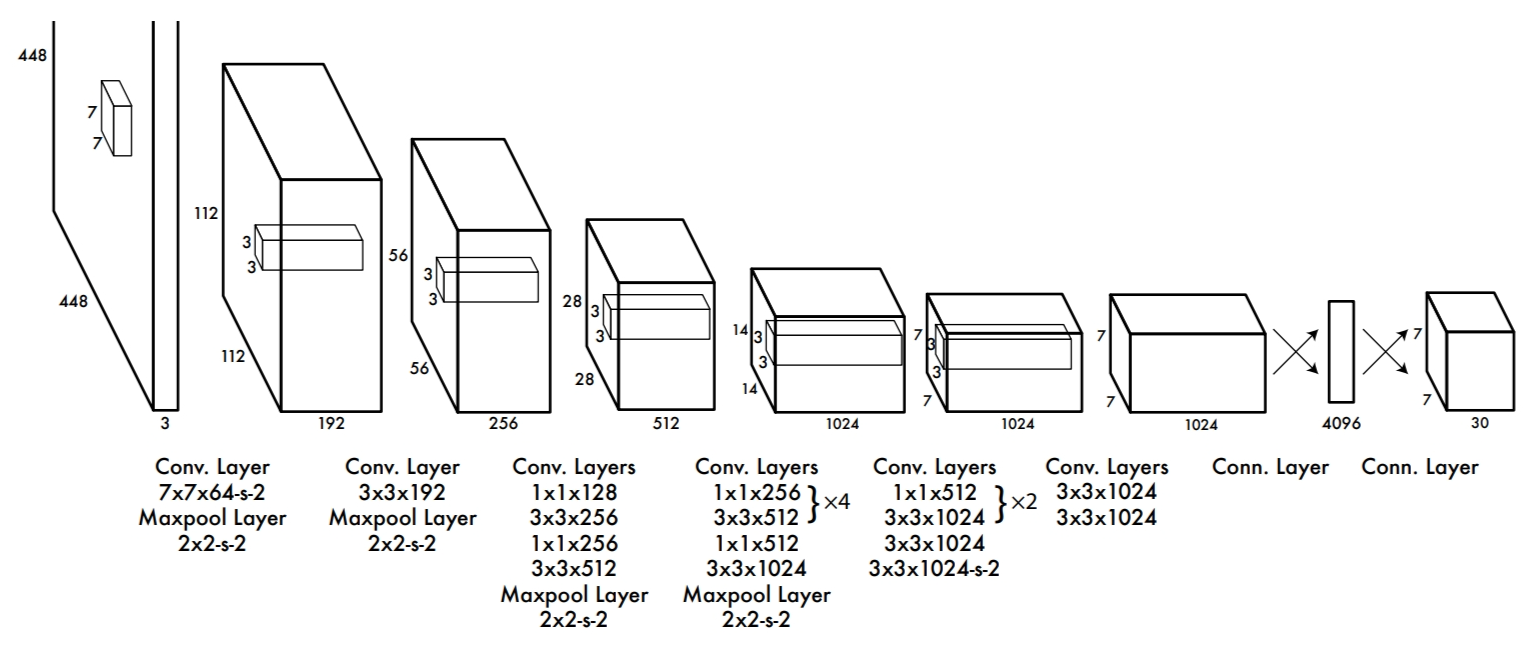
\includegraphics[scale=0.2]{resources/YOLO.png}
  \end{center}
  \caption[YOLO Architecture]{You Only Look Once Architecture}
  \label{fig:yolo architecture}
\end{figure}


\section{Object Relational Mapping (ORM)}
Object-Relational Mapping \cite{orm} เป็นการสร้างการสัมพันธ์ระหว่างฐานข้อมูลแบบ Relational กับโครงสร้างข้อมูลแบบ Object-Oriented 
ในการพัฒนาซอฟต์แวร์ เช่น เว็บแอปพลิเคชัน โดยที่ไม่ต้องเขียน SQL โดยตรงแต่สามารถใช้ภาษาโปรแกรมเพื่อจัดการกับข้อมูลแทน 
ซึ่งสามารถป้องกันการโจมตีแบบ SQL Injection ได้ ในกรณีที่กำหนดให้มีการเปลี่ยนแปลงในโครงสร้างข้อมูล 
คุณสมบัติหรือโครงสร้างข้อมูลในฐานข้อมูลจะถูกปรับเปลี่ยนตามในโครงสร้างของ Object ในโปรแกรม เป็นฐานข้อมูลแบบเสมือนในโปรแกรม 
โดยที่การจัดเก็บข้อมูลยังคงเป็นแบบ Relational เหมือนเดิม โดยไม่ต้องใช้ SQL Statements โดยตรง
\begin{figure}[h]
  \begin{center}
  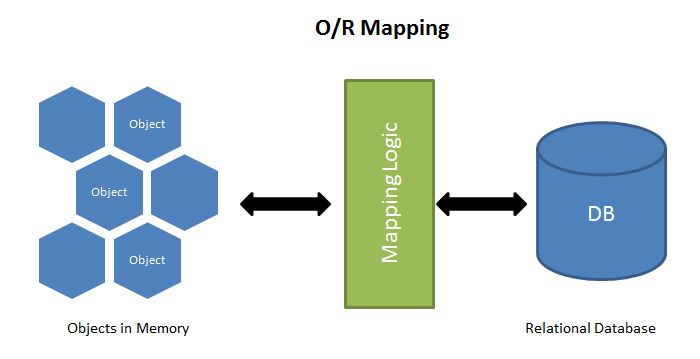
\includegraphics[scale=0.3]{resources/ORM.png}
  \end{center}
  \caption[Object Relational Mapping]{Object Relational Mapping}
  \label{fig:orm}
\end{figure}

\section{Model–View–Controller design pattern (MVC)}
Model-View-Controller \cite{mvc} เป็นรูปแบบโครงสร้างที่แยกแอปพลิเคชันออกเป็น 3 ส่วนหลักคือ: โมเดล (model), มุมมอง (view), 
และคอนโทรลเลอร์ (controller) แต่ละส่วนมีการสร้างขึ้นเพื่อจัดการด้านพัฒนาส่วนแอปพลิเคชันที่เฉพาะเจาะจง MVC 
เป็นหนึ่งในรูปแบบการพัฒนาเว็บตามมาตรฐานอุตสาหกรรมที่ถูกใช้บ่อยที่สุดเพื่อสร้างโครงงานที่สามารถเพิ่มและขยายขนาดในอนาคตได้ 
โดยที่ว่าเพื่อให้โปรแกรมนั้นดูเรียบง่ายต่อการแก้ไขจัดการ ซึ่งความหมายในแต่ละส่วนของ MVC นั้นได้แก่ 
\begin{enumerate}
  \item Model คือส่วนที่รับผิดชอบเกี่ยวกับข้อมูลและการประมวลผลทางด้านข้อมูลในแอปพลิเคชัน เช่น การเชื่อมต่อกับฐานข้อมูล การจัดการข้อมูล 
  และการประมวลผลทางข้อมูล เป็นต้น โดยที่ model มักจะเป็นตัวแทนของข้อมูลและสถานะของแอปพลิเคชัน
  \item View คือส่วนที่จะเป็นหน้าตาของโปรแกรมที่ผู้ใช้จะใช้งานจากส่วนนี้ ไม่ว่าจะเป็นการกรอกข้อมูล, ดูผลลัพธ์ หรือการมีปฏิสัมพันธ์กับผู้ใช้ 
  (User Interface) view จริง ๆ แล้วก็คือส่วนที่เรียกว่า GUI (Graphic User Interface) 
  \item Controller เป็นส่วนที่รับผิดชอบในการควบคุมและจัดการกับการกระทำที่เกิดขึ้นจากผู้ใช้งาน เช่น การรับข้อมูลจากผู้ใช้งาน, 
  การส่งข้อมูลไปยังโมเดลเพื่อประมวลผล, และการอัพเดตสถานะของ view ซึ่งโดยทั่วไปแล้ว controller จะเป็นตัวกลางที่เชื่อมต่อระหว่าง model 
  และ view โดยการควบคุมการทำงานของทั้งสอง 
\end{enumerate}
\begin{figure}[h]
  \begin{center}
  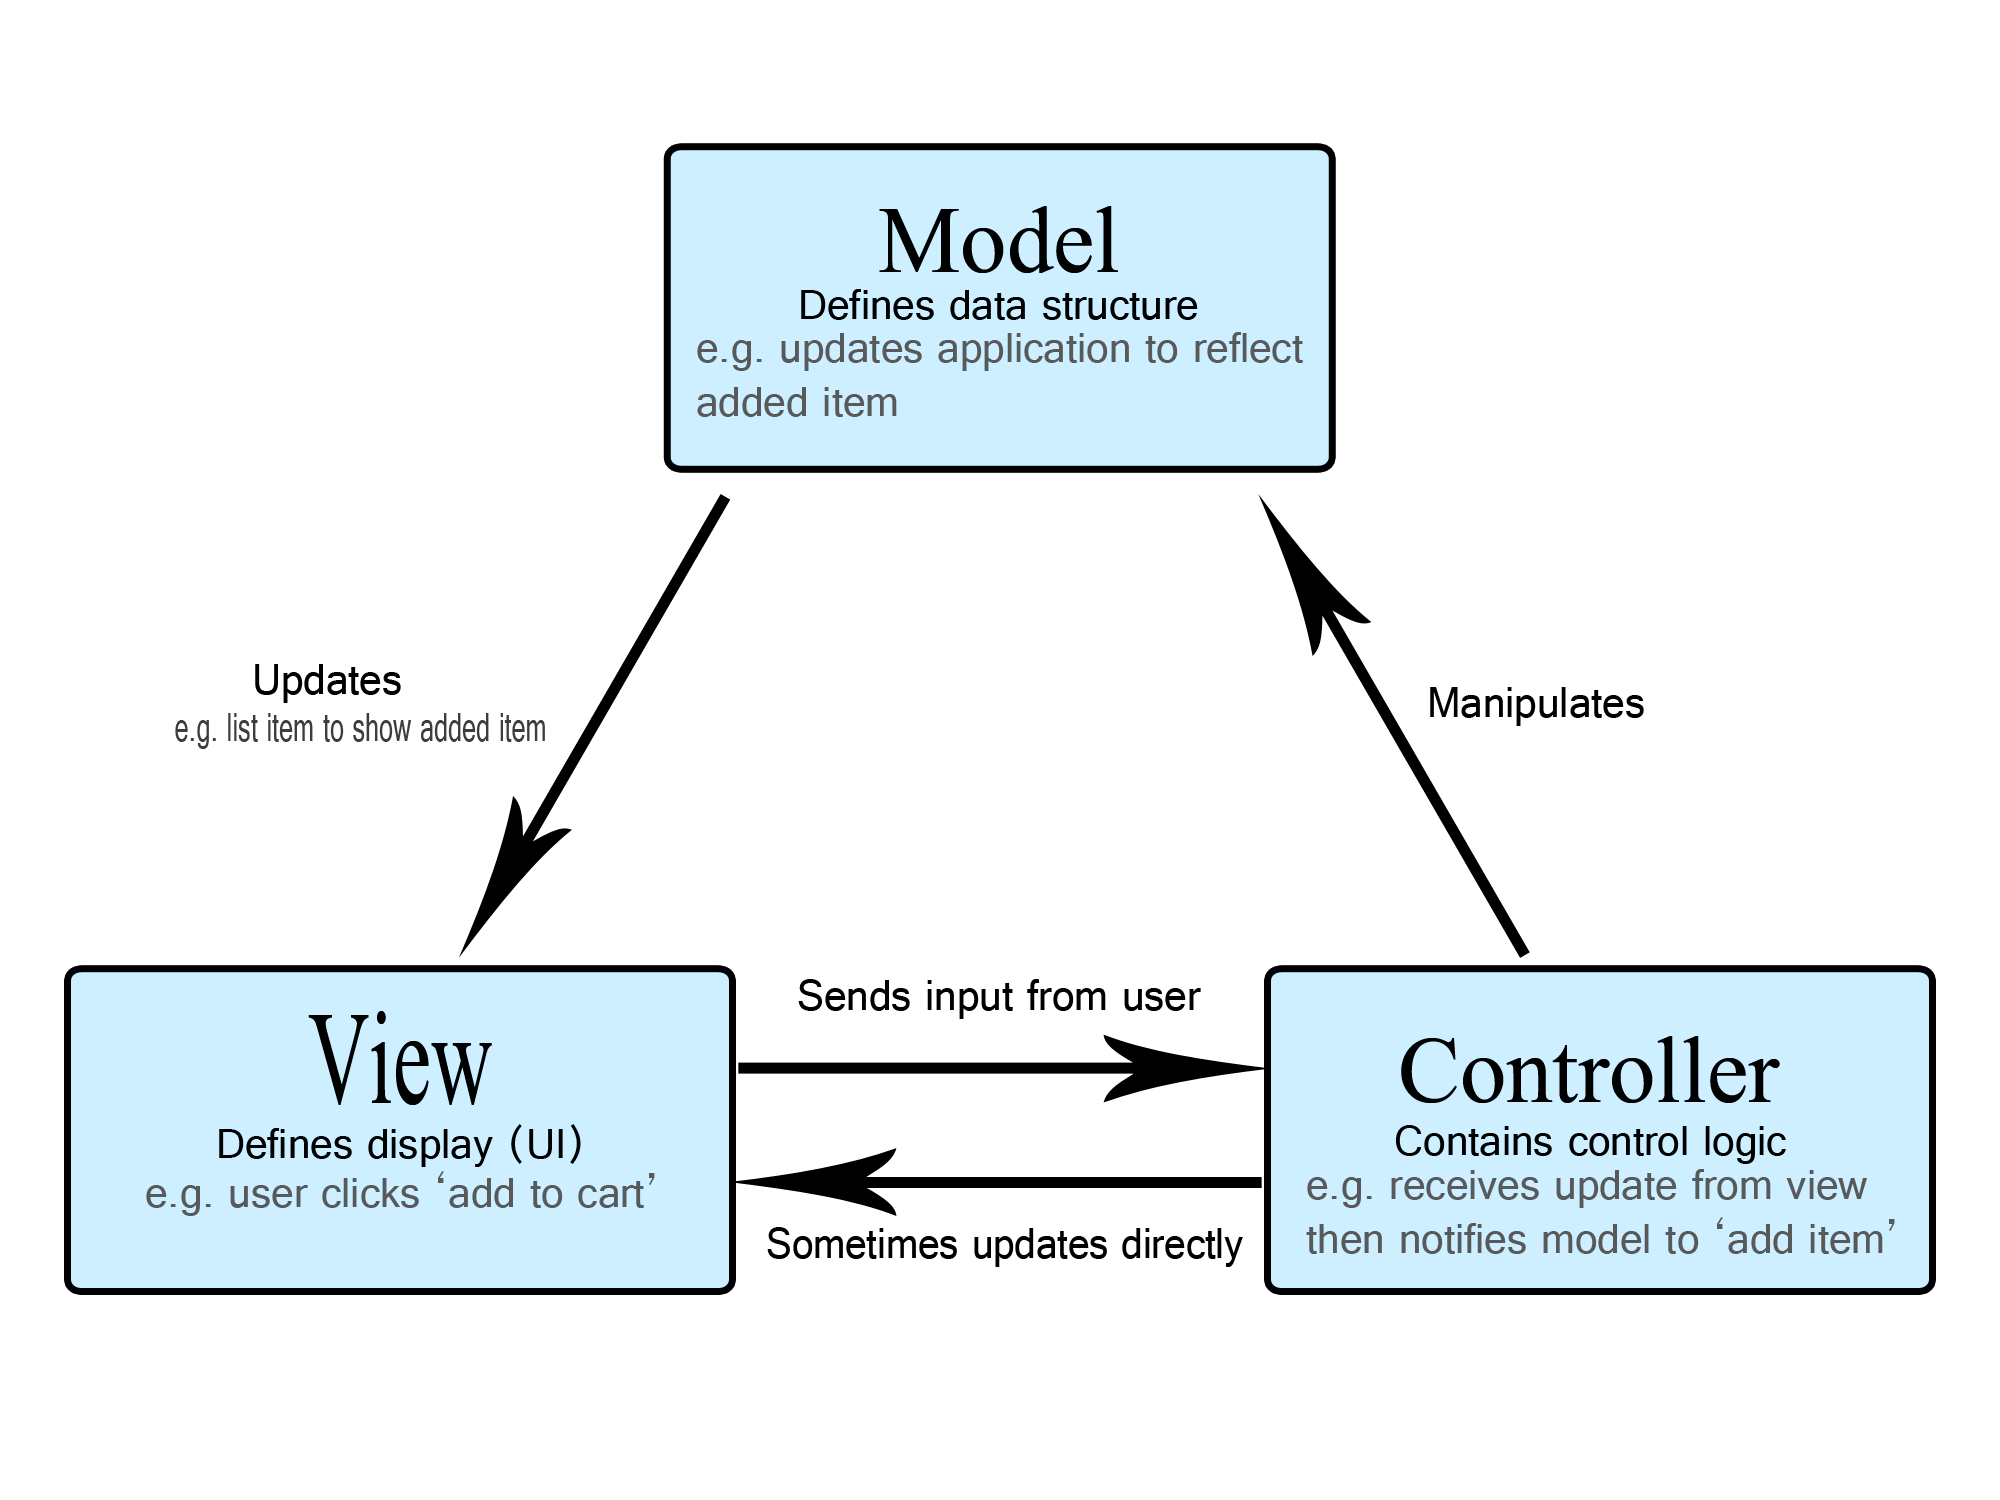
\includegraphics[scale=0.3]{resources/MVC.png}
  \end{center}
  \caption[Model-View-Controller]{Model-View-Controller Design Pattern}
  \label{fig:mvc}
\end{figure}

\section{Hypertext Transfer Protocol (HTTP)}
HTTP (Hypertext Transfer Protocol) เป็นโปรโตคอลสื่อสารที่ใช้ในการส่งข้อมูลระหว่างเครื่องคอมพิวเตอร์บนเครือข่ายอินเทอร์เน็ต โดย HTTP 
มีหน้าที่เป็นตัวกลางในการร้องขอและส่งข้อมูลระหว่างเว็บไซต์ (web servers) และเบราว์เซอร์ (web browsers) หรือแอปพลิเคชันอื่น ๆ 
ที่ใช้เครือข่ายอินเทอร์เน็ต 
\begin{itemize}
  \item API (Application Programming Interface) เป็นชุดของกฎและโครงสร้างข้อมูลที่กำหนดโดยโปรแกรมคอมพิวเตอร์เพื่อให้แอปพลิเคชันอื่น ๆ 
  สามารถสื่อสารและทำงานร่วมกันได้ ในเชิงพื้นฐาน API เป็นวิธีที่แอปพลิเคชันใช้เรียกใช้ฟังก์ชันหรือการบริการที่ให้มาจากแหล่งข้อมูลหรือบริการ
  ซึ่งอาจเป็นเซิร์ฟเวอร์เว็บ ฐานข้อมูล หรือแหล่งข้อมูลอื่น ๆ โดยทั่วไป API จะรองรับการร้องขอและการตอบกลับโดยใช้ฟอแมตที่เป็นรูปแบบมาตรฐาน เช่น 
  JSON (JavaScript Object Notation) หรือ XML (Extensible Markup Language) 
\end{itemize}

\section{Docker}
Docker \cite{docker} เป็นเทคโนโลยีคอนเทนเนอร์แพลตฟอร์มที่ช่วยในการสร้างและทำการงานร่วมกับคอนเทนเนอร์อย่างมีประสิทธิภาพ ด้วย Docker 
ผู้ใช้สามารถแยกแยะและแพคเกจแอปพลิเคชันพร้อมกับสิ่งที่เกี่ยวข้องทั้งหมด เช่น ไฟล์, ระบบปฏิบัติการ, ไลบรารี, และสิ่งอื่น ๆ 
ลงในคอนเทนเนอร์ได้อย่างเรียบง่าย ผู้ใช้สามารถสร้าง และรันคอนเทนเนอร์ได้โดยง่าย นอกจากนี้ Docker 
ยังช่วยลดปัญหาเกี่ยวกับสภาพแวดล้อมและการติดตั้งโปรแกรมที่ซับซ้อน ทำให้การพัฒนาและการทำงานของโปรแกรมมีประสิทธิภาพมากขึ้น 
\begin{figure}[h]
  \begin{center}
  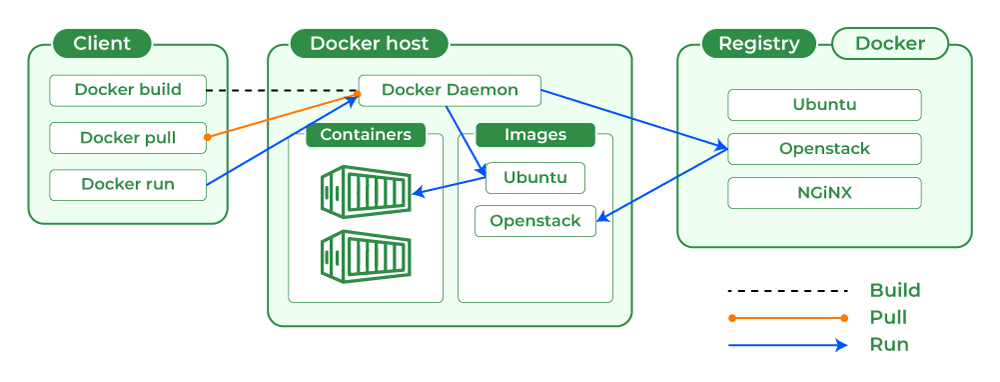
\includegraphics[scale=0.3]{resources/Docker.png}
  \end{center}
  \caption[Docker Architecture]{Docker Architecture}
  \label{fig:docker}
\end{figure}

\section{Interactive Website}
Interactive website \cite{interactive-web} คือ เว็บไซต์ที่สามารถให้ผู้ใช้งาน communicate หรือ interact เช่น การแสดงความคิดเห็น การตอบโต้กับตัวเว็บ 
การได้รับผลจากการกระทําในเว็บ ในลักษระที่เป็นมิตรต่อผู้ใช้ โดยปัจจุบัน มักใช้ animation sound picture audio etc. ประกอบ 
เพื่อให้มีความสนุกสนานและเพิ่มการเข้าถึงได้ง่ายของผู้ใช้ ทั้งนี้อาจทําเพื่อเก็บข้อมูลหลังจากการใช้งานเว็บไซต์ได้อีกด้วย ซึ่งดีกว่าเว็บที่มีแต่ตัวอักษร หรือ 
การแสดงผลเฉย ๆ ที่ได้รับข้อมูลทางฝ่ายเดียวอย่างแน่นอน

% \subsubsection{Subsubsection 1 heading goes here}
% Subsubsection 1 text

% \subsubsection{Subsubsection 2 heading goes here}
% Subsubsection 2 text

% \section{Third section}
% Section 3 text. The dielectric constant\index{dielectric constant}
% at the air-metal interface determines
% the resonance shift\index{resonance shift} as absorption or capture occurs
% is shown in Equation~\eqref{eq:dielectric}:

% \begin{equation}\label{eq:dielectric}
% k_1=\frac{\omega}{c({1/\varepsilon_m + 1/\varepsilon_i})^{1/2}}=k_2=\frac{\omega
% \sin(\theta)\varepsilon_\mathit{air}^{1/2}}{c}
% \end{equation}

% \noindent
% where $\omega$ is the frequency of the plasmon, $c$ is the speed of
% light, $\varepsilon_m$ is the dielectric constant of the metal,
% $\varepsilon_i$ is the dielectric constant of neighboring insulator,
% and $\varepsilon_\mathit{air}$ is the dielectric constant of air.

% \section{About using figures in your report}

% % define a command that produces some filler text, the lorem ipsum.
% \newcommand{\loremipsum}{
%   \textit{Lorem ipsum dolor sit amet, consectetur adipisicing elit, sed do
%   eiusmod tempor incididunt ut labore et dolore magna aliqua. Ut enim ad
%   minim veniam, quis nostrud exercitation ullamco laboris nisi ut
%   aliquip ex ea commodo consequat. Duis aute irure dolor in
%   reprehenderit in voluptate velit esse cillum dolore eu fugiat nulla
%   pariatur. Excepteur sint occaecat cupidatat non proident, sunt in
%   culpa qui officia deserunt mollit anim id est laborum.}\par}

% \begin{figure}[h]
%   \centering

%   \fbox{
%      \parbox{.6\textwidth}{\loremipsum}
%   }

%   % To include an image in the figure, say myimage.pdf, you could use
%   % the following code. Look up the documentation for the package
%   % graphicx for more information.
%   % \includegraphics[width=\textwidth]{myimage}

%   \caption[Sample figure]{This figure is a sample containing \gls{lorem ipsum},
%   showing you how you can include figures and glossary in your report.
%   You can specify a shorter caption that will appear in the List of Figures.}
%   \label{fig:sample-figure}
% \end{figure}

% Using \verb.\label. and \verb.\ref. commands allows us to refer to
% figures easily. If we can refer to Figures
% \ref{fig:walrus} and \ref{fig:sample-figure} by name in the {\LaTeX}
% source code, then we will not need to update the code that refers to it
% even if the placement or ordering of the figures changes.

% \loremipsum\loremipsum

% % This code demonstrates how to get a landscape table or figure. It
% % uses the package lscape to turn everything but the page number into
% % landscape orientation. Everything should be included within an
% % \afterpage{ .... } to avoid causing a page break too early.
% \afterpage{
%   \begin{landscape}
%   \begin{table}
%     \caption{Sample landscape table}
%     \label{tab:sample-table}

%     \centering

%     \begin{tabular}{c||c|c}
%         Year & A & B \\
%         \hline\hline
%         1989 & 12 & 23 \\
%         1990 & 4 & 9 \\
%         1991 & 3 & 6 \\
%     \end{tabular}
%   \end{table}
%   \end{landscape}
% }

% \loremipsum\loremipsum\loremipsum

% \section{Overfull hbox}

% When the \verb.semifinal. option is passed to the \verb.cpecmu. document class,
% any line that is longer than the line width, i.e., an overfull hbox, will be
% highlighted with a black solid rule:
% \begin{center}
% \begin{minipage}{2em}
% juxtaposition
% \end{minipage}
% \end{center}

% \section{\ifenglish%
% \ifcpe CPE \else ISNE \fi knowledge used, applied, or integrated in this project
% \else%
% ความรู้ตามหลักสูตรซึ่งถูกนำมาใช้หรือบูรณาการในโครงงาน
% \fi
% }

% อธิบายถึงความรู้ และแนวทางการนำความรู้ต่างๆ ที่ได้เรียนตามหลักสูตร ซึ่งถูกนำมาใช้ในโครงงาน

% \section{\ifenglish%
% Extracurricular knowledge used, applied, or integrated in this project
% \else%
% ความรู้นอกหลักสูตรซึ่งถูกนำมาใช้หรือบูรณาการในโครงงาน
% \fi
% }

% อธิบายถึงความรู้ต่างๆ ที่เรียนรู้ด้วยตนเอง และแนวทางการนำความรู้เหล่านั้นมาใช้ในโครงงาน

\chapter{\ifproject%
\ifenglish Project Structure and Methodology\else โครงสร้างและขั้นตอนการทำงาน\fi
\else%
\ifenglish Project Structure\else โครงสร้างของโครงงาน\fi
\fi
}

\import{chapters/approach/system}{system-overview.tex}
\import{chapters/approach/backend}{backend-overview.tex}
% TODO: UNCOMMENT THE FOLLOWING
% \chapter{\ifproject%
% \ifenglish Experimentation and Results\else การทดลองและผลลัพธ์\fi
% \else%
% \ifenglish System Evaluation\else การประเมินระบบ\fi
% \fi}

% TODO: DELETE THE FOLLOWING
\chapter{\ifenglish System Evaluation\else การประเมินระบบ\fi}

\ifenglish
\else
\section{การประเมินประสิทธิภาพซอฟต์แวร์}
ทดสอบประสิทธิภาพซอฟต์แวร์โดยจะมีการแบ่งส่วนในการทดสอบออกเป็นส่วน ๆ เพื่อให้รู้ว่าในแต่ละส่วนของซอฟต์แวร์ของเรานั้น 
ทำงานได้อย่างมีประสิทธิภาพหรือไม่ จึงสามารถแบ่งออกการประเมินได้เป็นดังนี้ 
\begin{enumerate}
    \item Classification model - เป็นการทดสอบเพื่อประเมินและตรวจสอบความเร็วในการประมวลผลเพื่อทำการ classify 
    ว่า object ใดเป็นป้ายที่สามารถจัดเก็บภาษีได้ รวมถึงในเรื่องของความแม่นยำในการ classify  
    \item Response time - เป็นการทดสอบเพื่อประเมินในเรื่องของความเร็วในการรับส่งข้อมูลระหว่าง client กับ application server  
\end{enumerate}

\section{การประเมินความพึงพอใจในการใช้งานระบบ}
ทดสอบความพึงพอใจในการใช้งานจะมีการแบ่งออกเป็นสองส่วน คือส่วนของแอปพลิเคชันในโทรศัพท์มือถือ กับส่วนของเว็บแอปพลิเคชัน 
โดยจะมีเกณฑ์การให้คะแนนอยู่ที่ 1 ถึง 5 โดยจะมีการให้คะแนนในเรื่องดังต่อไปนี้ 
\begin{enumerate}
    \item ความง่ายต่อการใช้งานของแอปพลิเคชัน 
    \item ความสะดวกในการใช้งานในตอนเริ่มต้นของแอปพลิเคชัน 
    \item ความดึงดูดในการใช้งานของแอปพลิเคชัน        
    \item ประโยชน์ที่มีของแอปพลิเคชัน 
\end{enumerate}

โดยที่ทั้ง 4 ข้อเป็นพิจราณาจากแนวคิดตาม The Four Elements of User Experience \cite{uxquantification} ที่ประกอบไป ด้วย 

\begin{enumerate}
    \item Usability ความใช้ง่ายในการใช้งาน เกี่ยวข้องกับสามารถในการใช้งาน รวมไปถึงความเหมาะสมการใช้งานกับผู้งานใช้ 
    \item Adaptability ความสามารถในงานปรับตัว กล่าวถึงระดับความยากง่ายของการใช้งานตั้งแต่จุดเริ่มต้น จนถึงจุดสิ้นสุดของระบบ โดยที่ผู้งานสามารถใช้งานได้อย่างคล่องแคล่ว 
    \item Desirability ความพึงพอใจ คือเมื่อใช้งานแล้วผู้ได้รับประสบการณ์ที่ดีในจากใช้งานของระบบ 
    \item Value คุณค่าของระบบ คือระบบที่ผู้ใช้เข้ามาใช้งานมีความสอดคล้องกับความต้องการของผู้ใช้ 
\end{enumerate}

โดยในส่วนของการประเมินความพึงพอใจในระบบทั้งในส่วนของเว็บไซต์และในส่วนของมือถือ ได้มีการเก็บผลการประเมินมาจากกลุ่มผู้ทดลองการใช้งานทั้ง 15 คน ซึ่งจะมีผลการประเมินเฉลี่ยเป็นดังรูป \ref{fig:evaluation-th}
\fi

\clearpage

\ifenglish
\insertPDFfigure{resources/eval/Average-Website-&-Mobile-Evaluation-by-Aspect.pdf}{Evaluation of System Satisfaction}{evaluation}
\else
\insertPDFfigure{resources/eval/Average-Website-&-Mobile-Evaluation-by-Aspect-thai.pdf}{ผลการประเมินความพึงพอใจในการใช้งานระบบ}{evaluation-th}

จากข้อมูลที่สามารถเห็นได้จากรูปภาพข้างต้น จะเห็นได้ว่าความพึงพอใจในการใช้งานระบบของโดยรวมในทุกด้านั้นมีค่าเฉลี่ยอยู่ที่ 4 ไปจนถึง 4.45 ซึ่งเป็นค่าที่สูงมาก แสดงให้เห็นว่าผู้ใช้งานมีความพึงพอใจในการใช้งานระบบของเราอย่างมาก โดยเราสามารถที่จะวิเคราะห์ในแต่ละด้านได้ดังนี้

\begin{enumerate}
    \item ระบบนี้มีประโยชน์ จากการประเมินของกลุ่มผู้ทดสอบทำให้เราทราบได้ว่าคะแนนของในส่วนเว็บไซต์กับในส่วนของมือถือนั้นจะมีค่าที่ใกล้เคียงกันอยู่ที่ประมาณ 4.3 เป็นการบ่งบอกได้ว่าระบบนี้มีประโยชน์ต่อสายตาของผู้ใช้งาน
    \item ระบบนี้ใช้งานง่าย ความง่ายของการใช้งานที่กลุ่มผู้ทดสอบได้ทดลองใช้ทั้งในส่วนของเว็บไซต์และในส่วนของมือถือ มีค่าเฉลี่ยอยู่ที่ 4.4 ซึ่งเป็นค่าที่สูงมาก แสดงให้เห็นว่าระบบนี้มีความง่ายในการใช้งานสำหรับผู้ที่ใช้งานที่ได้ทดลองใช้งานเป็นครั้งแรก
    \item ระบบนี้น่าเอาไปใช้ ความน่าไปใช้งานของระบบที่ได้รับคะแนนจากกลุ่มผู้ทดสอบที่ใช้งานทั้งในส่วนของเว็บไซต์และในส่วนของมือถือ มีค่าเฉลี่ยอยู่ที่ 4.4 ซึ่งเป็นค่าที่สูงมาก แสดงให้เห็นว่าระบบนี้น่าไปใช้งานสำหรับผู้ที่เข้ามาทดลองใช้งาน
    \item ระบบมีความสนุก ความสนุกในการใช้งานระบบที่ได้รับคะแนนจากกลุ่มผู้ทดสอบที่ใช้งานทั้งใน\\ ส่วนของเว็บไซต์และในส่วนของมือถือ มีค่าเฉลี่ยอยู่ที่ 4 ซึ่งเป็นการบ่งบอกว่าระบบนี้มีความสนุกในการใช้งานที่น้อยกว่าในด้านที่เหลือ ควรที่จะมีการปรับปรุงให้ดียิ่งขึ้น เพื่อให้ผู้ที่เข้ามาใช้งานนั้นรู้สึกสนุกเมื่อเข้ามาใช้งาน
\end{enumerate}
\fi
% \ifproject
% \include{chapters/conclusion}
% \fi

\bibliography{ScreetnerReport}

% \ifproject
% \normalspacing
% \appendix
% \include{chapters/appendix}

%% Display glossary (optional) -- need glossary option.
% \ifglossary\glossarypage\fi

%% Display index (optional) -- need idx option.
% \ifindex\indexpage\fi

% \begin{biosketch}
% \begin{center}
%   \includegraphics[width=1.5in]{mugshot.jpg}
% \end{center}
% Your biosketch goes here. Make sure it sits inside
% the \texttt{biosketch} environment.
% \end{biosketch}
% \fi % \ifproject
\end{document}
